\subsection{Güte des Selektivverstärkers}
\begin{table}[h]
	\begin{center}
		\begin{tabular}{ccc}
			Frequenz [kHz] & Ausgansspannung $U_aus$ [mV]\\ \hline
			30	&31\\
			31	&38\\
			32	&52\\
			33	&78\\
			34	&155\\
			34,2&185\\
			34,4&237\\
			34,6&315\\
			34,8&480\\
			35	&755\\
			35,2&685\\
			35,4&430\\
			35,6&300\\
			35,8&220\\
			36	&180\\
			37	&88\\
			38	&58,5\\
			39	&44\\
			40	&35,5\\
		\end{tabular}
		\caption{Güte des Selektivfilters}
		\label{taba}
	\end{center}
\end{table}
\begin{figure}[h]
		\begin{center}
		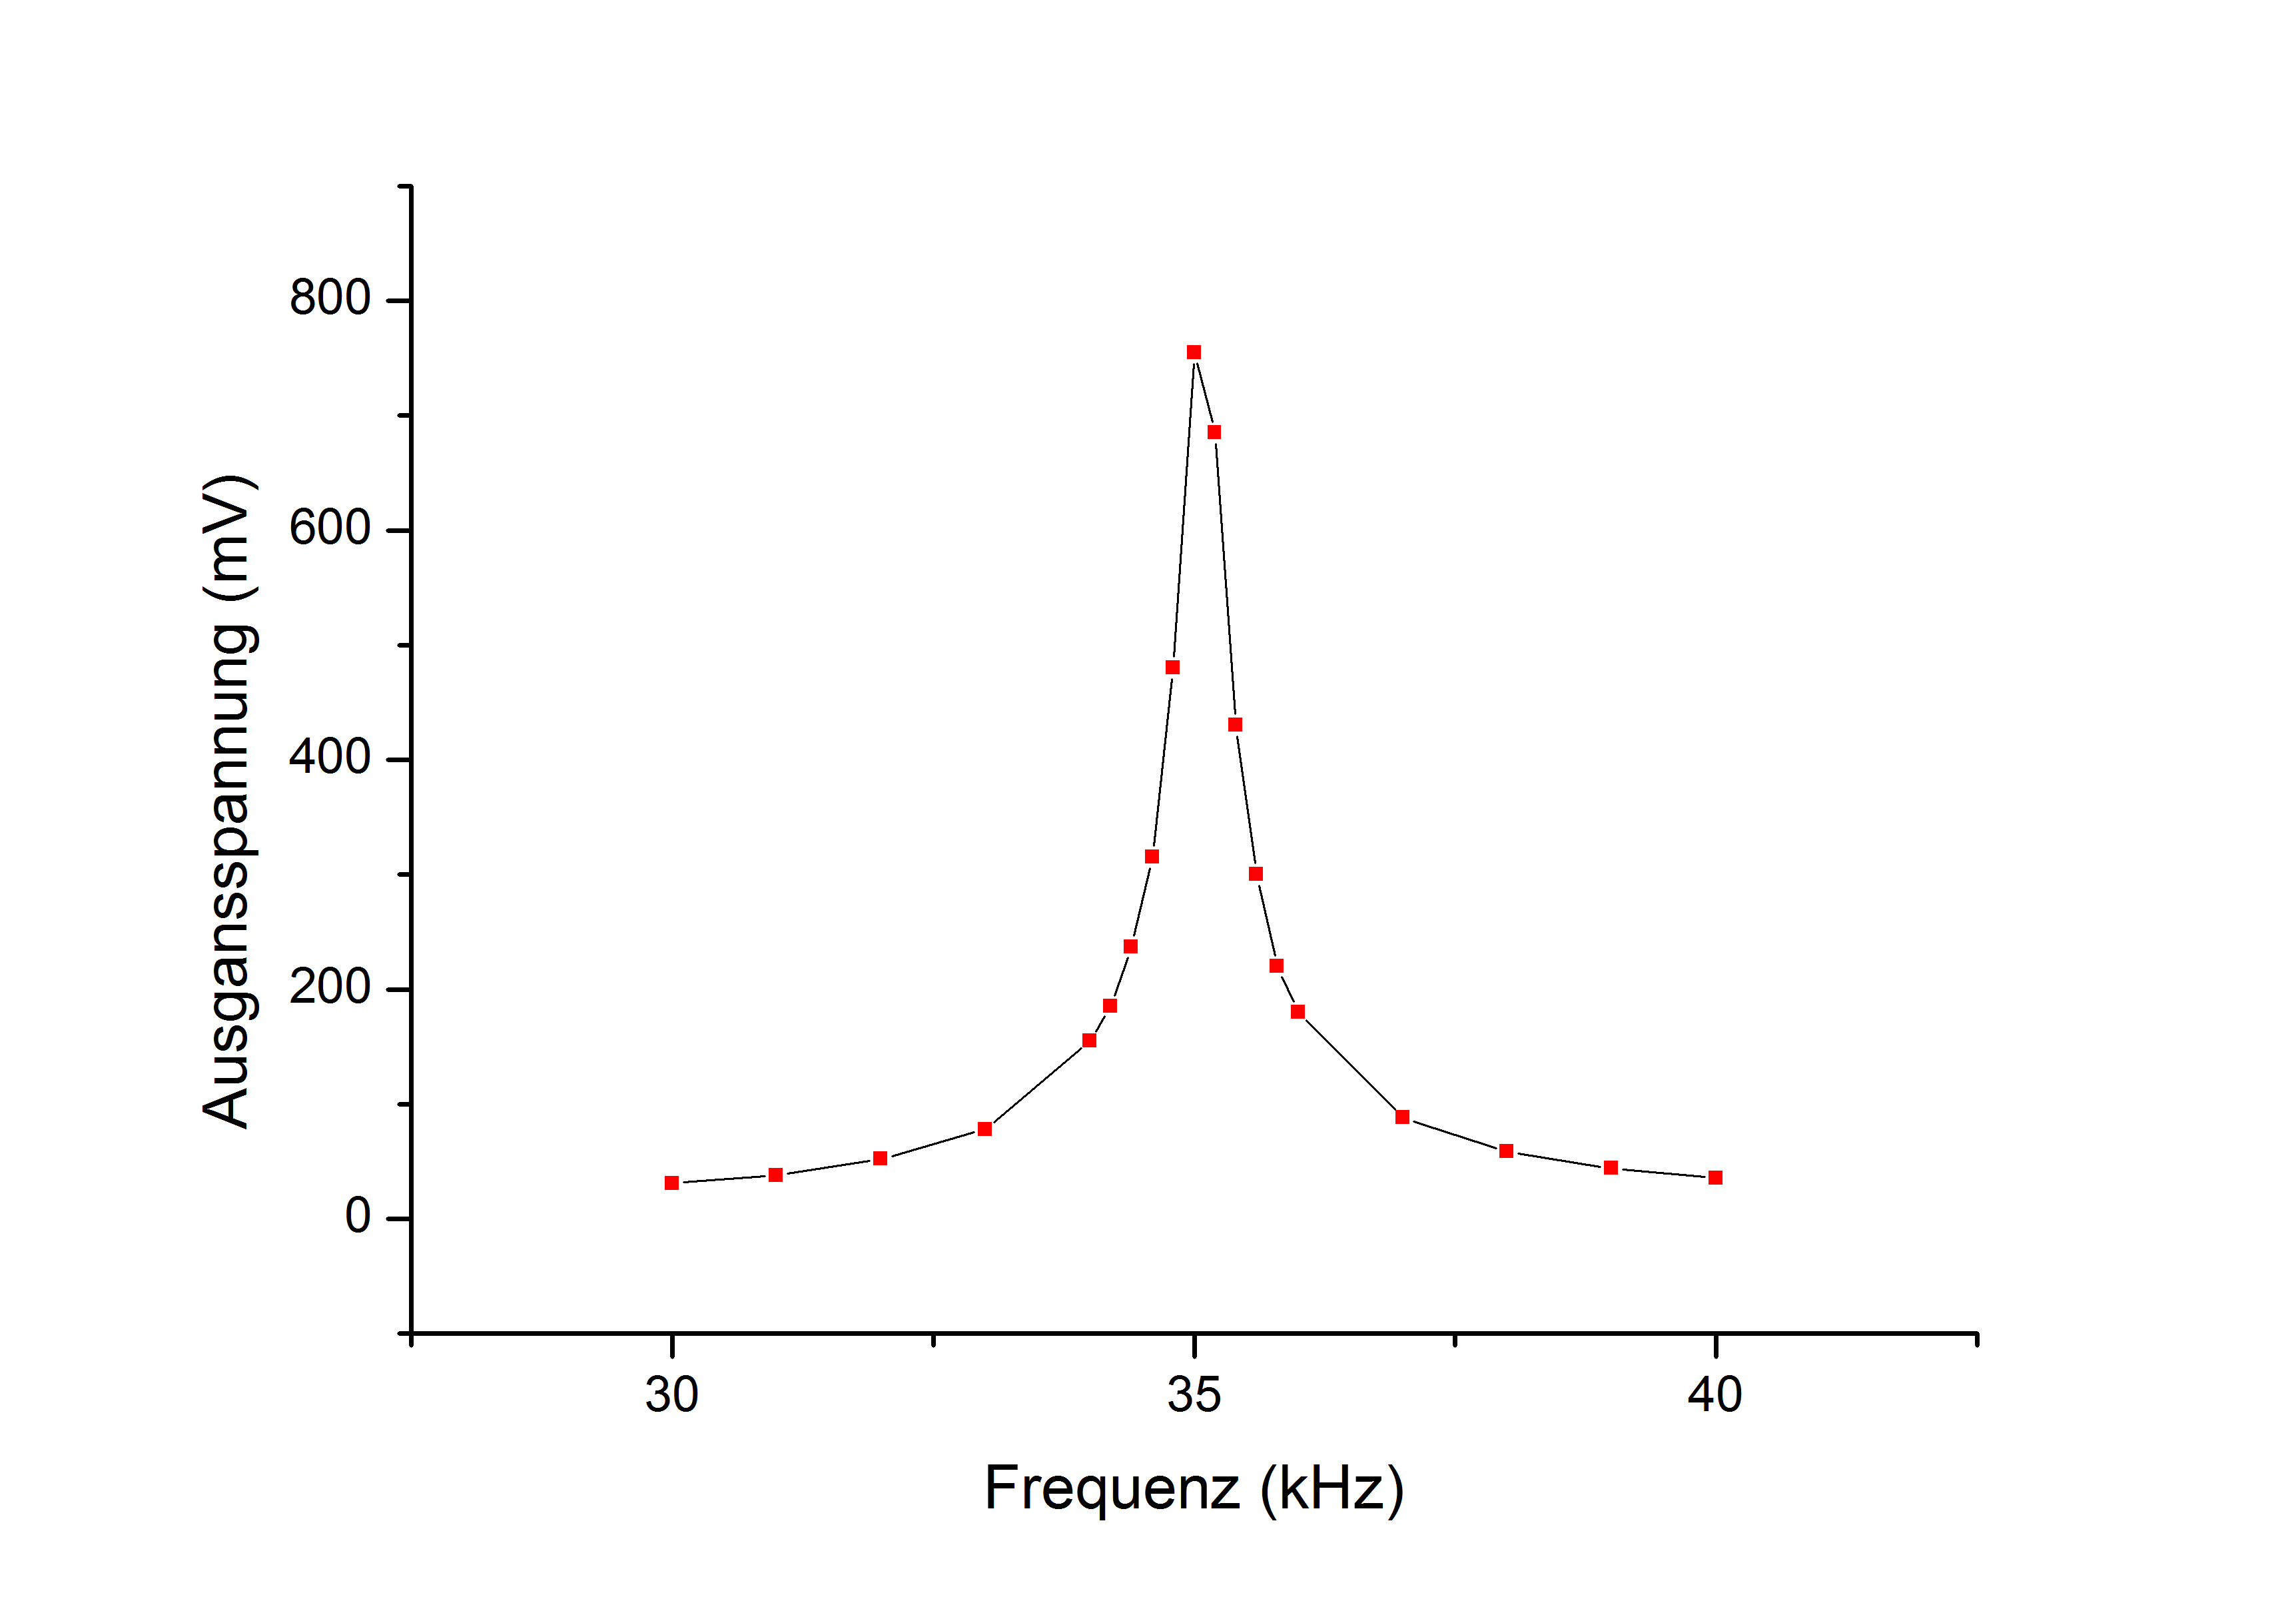
\includegraphics[scale=0.4]{gute.jpg}
		\caption{Güte des Selektivverstärkers}
		\label{gute}
		\end{center}	
\end{figure}

Aus dem Graph \ref{gute} lassen sich die Werte $\nu_-=34,8$ und $\nu_+=35,3$ ablesen. Aus \eqref{eqn:engute} ergibt sich eine Güte von q=70.

\subsection{Probe 1}
Bei der ersten Probe Handelt es sich um $Nd_2O_3$ mit folgenden Werten:
\begin{align*}
&J=\frac92&
&g_J=\frac{8}{11}&
&\rho=7,24\frac{g}{cm^3}&
&N=1,296*10^{26}m^{-3}&
\end{align*}
\\
Daraus ergibt sich aus dem Curie'schen Gesetz \eqref{eqn:curie}
$\chi=1,511*10^{-5}$
\begin{table}[ht]
	\begin{center}
		\begin{tabular}{cc}
			Brückenspannung $U_B$ [mV] & $\Delta R$ [m$\Omega$]\\ \hline
			2,2	&90\\
			1,7	&50\\
			1,75&85\\
			1,75&50\\
		\end{tabular}
		\caption{$C_6O_{12}Pr_2$}
		\label{tab1}
	\end{center}
\end{table}
Aus der Tabelle \ref{tab1} ergeben sich die gemittelten Werte
\begin{align*}
&R_3=2564,25m\Omega&
&U_{Br}=3,25mV&
&\Delta R=121,25m\Omega&
\end{align*}
Nach \eqref{eqn:chibrucke} lässt sich über die Brückenspannung
$\chi=1,699*10^{-3}$
berechnen.
\\
Aus der Widerstandsmessung ergibt sich nach \eqref{eqchir}
$\chi=1,022$


\subsection{Probe 2}
Bei der zweiten Probe Handelt es sich um $Gd_2O_3$ mit folgenden Werten:
\begin{align*}
&J=\frac72&
&g_J=2&
&\rho=7,40\frac{g}{cm^3}&
&N=1,229*10^{26}m^{-3}&
\end{align*}
Daraus ergibt sich nach \eqref{eqn:curie}
$\chi=6,897*10^{-5}$
\begin{table}[h]
	\begin{center}
		\begin{tabular}{cc|ccc}
			Brückenspannung $U_B$ [mV]&$\chi_{U}*10^-3$ & $\Delta R$ [m$\Omega$]&$R_3[\text{m}\Omega]$&$\chi_R*10^{-3}$\\ \hline
			3,5	&4,493&140&2555&3,165\\
			2,8	&3,594&90&2552&2,037\\
			3	&3,851&100&2550&2,265\\
			3,7	&4,750&155&2600&3,444
		\end{tabular}
		\caption{$Nd_2O_3$}
		\label{tab2}
	\end{center}
\end{table}
Aus der Tabelle \ref{tab2} ergeben sich die gemittelten Werte
\begin{align*}
&R_3=2553,75m\Omega&
&U_{Br}=17,25mV&
&\Delta R=770m\Omega&
\end{align*}
Nach \eqref{eqn:chibrucke} lässt sich über die Brückenspannung
$\chi=5,891*10^{-3}$
berechnen.
\\
Aus der Widerstandsmessung ergibt sich nach \eqref{eqchir}
$\chi=4,254$


\subsection{Probe 3}
Bei der dritten Probe Handelt es sich um $Dy_2O_3$ mit folgenden Werten:
\begin{align*}
&J=\frac{15}{2}&
&g_J=\frac43&
&\rho=7,80\frac{g}{cm^3}&
&N=1,259*10^{26}m^{-3}&
\end{align*}
Daraus ergibt sich nach \eqref{eqn:curie} 
$\chi=1,271*10^{-4}$
\begin{table}[h]
	\begin{center}
		\begin{tabular}{c|ccc}
				a	&Radius						&Höhe	&Masse \\ \hline
			Arm		&$(6,850\pm1,765)*10^{-3}$	&0,142	&0,01447$\pm$53,96%\\
			Kopf	&$(1,23\pm0,324)*10^{-2}$	&0,053	&0,01744$\pm$55,11%\\
			Torso	&$(1,82\pm0,25)*10^{-2}$	&0,0975	&0,06991$\pm$31,85%\\
			Bein	&$(8,375\pm1,395)*10^{-3}$	&0,149	&0,02270$\pm$37,00%
		\end{tabular}
		\caption{Messdaten der Trägheitspuppe}
		\label{tab:puppe}
	\end{center}
\end{table}
Aus der Tabelle \ref{tab3} ergeben sich die gemittelten Werte
\begin{align*}
&R_3=2553,75m\Omega&
&U_{Br}=36,125mV&
&\Delta R=1646,25m\Omega&
\end{align*}
Nach \eqref{eqn:chibrucke} lässt sich über die Brückenspannung
$\chi=11,029*10^{-3}$
berechnen.
\\
Aus der Widerstandsmessung ergibt sich nach \eqref{eqchir}
$\chi=8,132$